\documentclass[10pt,a4paper]{article}
\usepackage[T1]{fontenc}
\usepackage{lmodern}
\usepackage[margin=22mm]{geometry}
\usepackage{amsmath,amssymb,booktabs,graphicx,microtype}
\usepackage{xcolor}
\usepackage[colorlinks=true,urlcolor=blue!55!black,linkcolor=blue!45!black,citecolor=blue!45!black]{hyperref}
\usepackage{enumitem}
\setlist{nosep,leftmargin=*}
\setlength{\parindent}{0pt}
\setlength{\parskip}{5pt}
\setlength{\emergencystretch}{2em}
\hypersetup{pdftitle={Adversarial Training via Min-Max Optimization},pdfauthor={Anna Makridou and Alexandros Fourtounis},pdfsubject={Corrected CS-573 course project; CIFAR-10 study, seed 42}}
\newcommand{\eps}{\varepsilon}
\newcommand{\CE}{\operatorname{CE}}
\begin{document}
\begin{center}
{\LARGE\bfseries Adversarial Training via\\[3pt] Min-Max Optimization\par}
\vspace{8pt}
{\large Anna Makridou \quad Alexandros Fourtounis\par}
Computer Science Department, University of Crete\\
CS-573: Optimization Methods \quad | \quad Course project\\
Corrected report, 9 October 2026
\end{center}
\vspace{3pt}
\begin{abstract}
We compare clean continuation and mixed adversarial fine-tuning of a convolutional
classifier on CIFAR-10. Both branches start from the same clean pre-training
checkpoint and receive the same number of optimizer updates. Images remain in
pixel space during attack generation, and validation data select the checkpoints.
On all 10,000 test images, PGD-20 with five random restarts at $\eps=4/255$ yields
35.82\% robust accuracy for the adversarial branch and 1.14\% for the clean control.
Clean accuracy decreases from 78.70\% to 70.59\%. The comparison therefore shows a
measured accuracy--robustness tradeoff for this protocol. Results cover one seed
and four perturbation budgets; they do not establish statistical significance,
optimal hyperparameters, or robustness beyond the evaluated attacks.
\end{abstract}

\section{Scope and motivation}
Adversarial training frames learning as optimization against input perturbations.
Goodfellow et al. introduced a gradient-sign attack and studied adversarial
training~\cite{goodfellow}. Madry et al. developed the robust-optimization
formulation and its PGD-based approximation~\cite{madry}. This project implements
these ideas in PyTorch and measures the effect of mixed adversarial fine-tuning
relative to an equally long clean continuation.

The research question is narrow: after a shared clean pre-training stage, how do
clean test accuracy and empirical PGD robustness differ between the two branches?
The experiment compares a clean control with a loss containing equal clean and
adversarial weights. It does not compare every supported objective or establish
that pre-training is necessary.

This report supersedes the numerical interpretation of the original course
report. The earlier implementation clipped normalized tensors to $[0,1]$, which
did not enforce the stated pixel-space threat model. Its historical experiments
lack the checkpoints and logs required for verification. The results below come
from the corrected implementation and a newly completed full-data run. Authorship
is retained for the joint course project; no division of individual contributions
is asserted here.

\section{Data and model}
CIFAR-10 contains RGB images of size $32\times32$ in ten classes~\cite{cifar}.
We reserve 5,000 of the official 50,000 training images for validation and train
on the remaining 45,000. A seeded permutation determines this split. All 10,000
official test images are used only for the final analyses. Training uses random
crops with four-pixel padding and random horizontal flips; validation and test
images receive no augmentation.

The CNN has four $3\times3$ convolutions with channels
$3\rightarrow64\rightarrow128\rightarrow256\rightarrow256$, each followed by
batch normalization and ReLU. A $2\times2$ max-pooling operation follows each pair
of convolutions. The resulting $256\times8\times8$ features feed a
$16{,}384\rightarrow512\rightarrow10$ classifier with ReLU and dropout of 0.5.
The model has 9,356,554 trainable parameters. Input tensors stay in $[0,1]$;
channel normalization occurs inside the model, with means
$(0.4914,0.4822,0.4465)$ and standard deviations $(0.2023,0.1994,0.2010)$.

\newpage
\section{Optimization and attack procedure}
For adversarial loss weight $r$, the implemented training objective is
\begin{equation}
\min_\theta\;\mathbb{E}_{(x,y)}\!\left[
(1-r)\CE(f_\theta(x),y)
+r\max_{z\in\mathcal C(x)}\CE(f_\theta(z),y)\right],
\end{equation}
where $\mathcal C(x)=\{z:\|z-x\|_\infty\leq\eps,\;z\in[0,1]^d\}$.
The clean control uses $r=0$; mixed fine-tuning uses $r=0.5$. Both losses are
computed on the same batch, so the weight is not a fraction of examples replaced.
The code also supports $r=1$, but pure adversarial training is not evaluated in
this full comparison.

PGD approximately solves the inner maximization by projected gradient ascent:
\begin{align}
z_0 &= \Pi_{\mathcal C(x)}(x+u),\qquad u_i\sim\mathcal U(-\eps,\eps),\\
z_{t+1} &= \Pi_{\mathcal C(x)}\!\left(z_t+
\alpha\,\operatorname{sign}(\nabla_z\CE(f_\theta(z_t),y))\right).
\end{align}
Projection clamps each perturbation coordinate to $[-\eps,\eps]$ and then clamps
pixels to $[0,1]$. Training retains the highest-loss candidate among the clean
image and visited attack points. Evaluation instead prioritizes any
misclassified candidate, retaining it across steps and restarts, and breaks ties
by cross-entropy. This prevents a later step from undoing an earlier successful
attack. PGD is an approximate solver; no global maximizer is assumed.

During attack generation, dropout is disabled and batch statistics are frozen.
Gradients are requested only for the input; the caller's module modes are then
restored. Training updates use the usual training mode. FGSM is implemented and
tested as one projected gradient-sign step, but is not used for the reported table.

\section{Experimental protocol}
The fixed protocol is recorded in \texttt{experiments/full.json}. Seed 42 controls
initialization, the data split, and random generators. Batch size is 128, with
352 optimizer steps per epoch. SGD uses momentum 0.9 and weight decay $5\times10^{-4}$.

\begin{center}
\small
\begin{tabular}{@{}lccc@{}}
\toprule
 & Pre-training & Clean control & Mixed fine-tuning\\
\midrule
Epochs & 10 & 5 & 5\\
Initial learning rate & 0.01 & 0.001 & 0.001\\
Decay after epochs & 6, 9 & 3, 4 & 3, 4\\
Decay factor & 0.1 & 0.1 & 0.1\\
Adversarial loss weight & 0 & 0 & 0.5\\
Training PGD steps & --- & --- & 10\\
Training budget / step size & --- & --- & $4/255$ / $2/255$\\
Optimizer updates & 3,520 & 1,760 & 1,760\\
\bottomrule
\end{tabular}
\end{center}

Both branches load the final epoch-10 pre-training weights, then start fresh
optimizers and schedulers. They share the validation split and allotted update
count. Their computational cost differs because mixed training generates attacks
and computes both losses. They are not matched for wall time or forward passes.

Validation runs each epoch. The clean control is selected by clean validation
accuracy; the adversarial branch by PGD-10 validation robustness with one random
restart at $4/255$ and step size $2/255$. Both selected checkpoints are from
branch epoch 4; the clean branch ties at epoch 5, and the earlier checkpoint is
retained. Test measurements never determine checkpoint selection.

Final evaluation uses an untargeted white-box $L_\infty$ PGD attack: 20 steps,
five random restarts, step size $2/255$, and budgets $2/255$, $4/255$, $6/255$, and
$8/255$. Each budget is evaluated on all 10,000 test images.

\newpage
\section{Results}
Clean accuracy is the fraction correctly classified before attack. Robust
accuracy is the fraction correct both before and after attack. Attack success
rate (ASR) is conditional on clean correctness:
\begin{equation}
A_{\rm robust}=100\frac{n_{\rm clean\;and\;attacked\;correct}}{N},\qquad
\mathrm{ASR}=100\frac{n_{\rm clean\;correct}-n_{\rm clean\;and\;attacked\;correct}}
{n_{\rm clean\;correct}}.
\end{equation}
The clean input is a valid evaluation candidate, so robust accuracy cannot exceed
clean accuracy. ASR is undefined if no clean images are classified correctly.

\begin{table}[h!]
\centering
\caption{Full test results, seed 42. All values are percentages; PGD-20 uses five
restarts. Clean accuracy is 78.70\% for the control and 70.59\% for the adversarial branch.}
\label{tab:results}
\begin{tabular}{@{}ccccc@{}}
\toprule
 & \multicolumn{2}{c}{Robust accuracy} & \multicolumn{2}{c}{ASR}\\
\cmidrule(lr){2-3}\cmidrule(l){4-5}
Budget & Clean control & Adversarial & Clean control & Adversarial\\
\midrule
$2/255$ & 21.69 & 54.63 & 72.44 & 22.61\\
$4/255$ & 1.14 & 35.82 & 98.55 & 49.26\\
$6/255$ & 0.05 & 20.50 & 99.94 & 70.96\\
$8/255$ & 0.00 & 10.42 & 100.00 & 85.24\\
\bottomrule
\end{tabular}
\end{table}

\begin{figure}[h!]
\centering
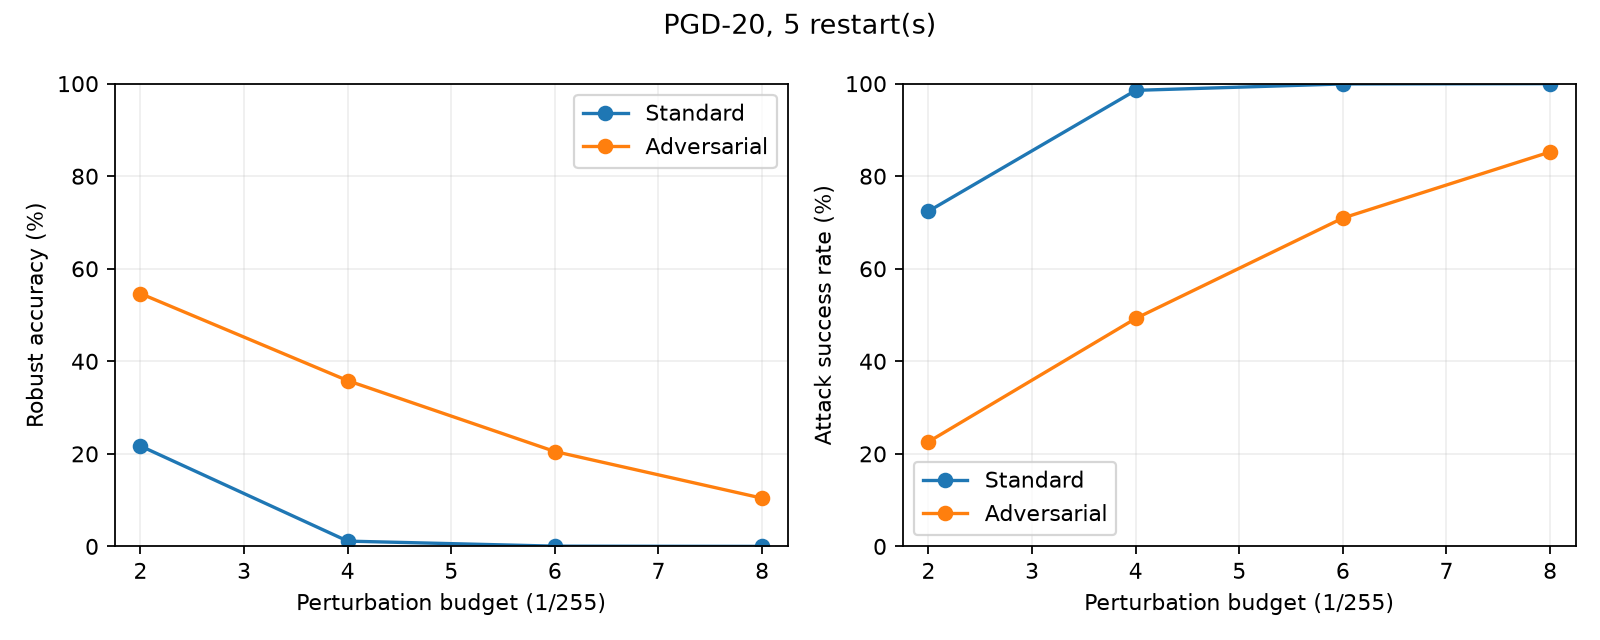
\includegraphics[width=\linewidth]{docs/results/full_cuda/comparison.png}
\caption{Measured robust accuracy and attack success rate. ``Standard'' denotes
the clean continuation control. The figure is generated
from the saved test measurements; the two ASR curves use their respective sets
of clean-correct images as denominators.}
\label{fig:comparison}
\end{figure}

At the training budget of $4/255$, mixed fine-tuning improves observed robust
accuracy by 34.68 percentage points and reduces clean accuracy by 8.11 points.
The adversarial branch has 3,582 robust-correct examples, compared with 114 for
the control. These are aggregate counts; they do not identify which individual
images change correctness between models. ASR falls by 49.30 percentage points,
computed from the unrounded measurements.

The adversarial branch has higher measured robust accuracy at all four tested
budgets. Its robust accuracy still falls to 10.42\% at $8/255$. These observations
support a tradeoff for the evaluated setting, rather than a claim of general
attack resistance. The experiment does not support the original report's claim
of simultaneous improvement in clean and robust accuracy.

\newpage
\section{Verification and reproducibility}
The full run completed on native Windows with an NVIDIA GeForce RTX 4060, Python
3.13.14, PyTorch 2.11.0+cu128, torchvision 0.26.0+cu128, NumPy 2.5.2, and
Matplotlib 3.11.2. The data loader used zero worker processes and the environment
set \texttt{OMP\_NUM\_THREADS=4}. Exact installed package versions are recorded in
\texttt{requirements-lock-windows.txt}; platform-specific commands are in
\texttt{docs/windows-guide.md}.

Eighteen regression tests pass. They cover attack bounds, zero-budget identity,
gradient calculations, parameter-gradient and model-mode preservation, metric
counts, checkpoint serialization, disjoint data splits, training and analysis,
atomic writes, experiment locking, and epoch-boundary recovery. An independent
small reference calculation checks PGD, and a CPU test compares resumed weights
with uninterrupted training. These tests support implementation correctness;
they are not a separate robustness benchmark.

Each training stage saves its configuration and per-epoch history. Selected
checkpoints have SHA-256 identifiers; both branches' records contain the same
pre-training hash. The export verifies those files, metric counts, and the
source/protocol hashes saved at launch. Portable records, histories, the summary,
and comparison plot are available in \texttt{docs/results/full\_cuda/}. Full
checkpoints remain in the local experiment directory and in a separate backup;
they are excluded from the source distribution because of their size.

The runner writes checkpoints atomically, protects an experiment from concurrent
writers, and restores optimizer, scheduler, random-generator, and data-loader
states when resuming at an epoch boundary. Analysis restarts after interruption.
Seeds improve repeatability, but identical floating-point results across different
devices or library versions are not guaranteed.

\section{Interpretation and limitations}
The clean continuation controls for extra optimizer updates after pre-training.
For this run, replacing the clean objective with the mixed objective increases
empirical PGD robustness at the cost of clean accuracy. The comparison does not
isolate equal computation, nor does it establish that the selected loss weight,
learning rates, training length, or architecture are optimal.

Only seed 42 is reported, so variation across initializations and validation
splits is unknown. Evaluation uses one attack family, one loss, and a fixed step
size. More steps and restarts than training improve the scrutiny of the same
attack family, but do not replace independent attack suites or prove absence of
gradient masking. There is no robustness certificate or deployment-safety claim.
The earlier subset pilot is retained separately and is not pooled with the full
test results.

This completes a reproducible course-project comparison of clean continuation
and mixed adversarial fine-tuning. Further seeds and independent attacks are
natural extensions of this study. The current evidence supports reporting the
measured tradeoff with its exact protocol and single-seed scope.

\begin{thebibliography}{9}
\small
\bibitem{goodfellow} I. J. Goodfellow, J. Shlens, and C. Szegedy.
\textit{Explaining and Harnessing Adversarial Examples}. 2015.
\href{https://arxiv.org/abs/1412.6572}{arXiv:1412.6572}.
\bibitem{madry} A. Madry, A. Makelov, L. Schmidt, D. Tsipras, and A. Vladu.
\textit{Towards Deep Learning Models Resistant to Adversarial Attacks}. ICLR, 2018.
\href{https://arxiv.org/abs/1706.06083}{arXiv:1706.06083}.
\bibitem{cifar} A. Krizhevsky. \textit{Learning Multiple Layers of Features from
Tiny Images}. Technical report, University of Toronto, 2009.
\href{https://www.cs.toronto.edu/~kriz/cifar.html}{CIFAR dataset and report}.
\end{thebibliography}
\end{document}
